\documentclass{article}

\usepackage[vmarginratio=1:1,a4paper,body={6.5in, 9.5in}]{geometry}

\usepackage[T2A]{fontenc}
\usepackage[utf8]{inputenc}
\usepackage[russian]{babel}

\usepackage{amsmath}
\usepackage{amssymb}
\usepackage{amsfonts}
\usepackage{amsthm}
\usepackage{color}

\usepackage{hyperref}
\usepackage{graphicx}


\title{Control moment gyroscope}
\author{}
\date{}

\begin{document}

\maketitle

\section{Симметричный гиродин}
\subsection{Вводная и способ вывода Лагранжиана}

\begin{figure}[!ht]
\centering
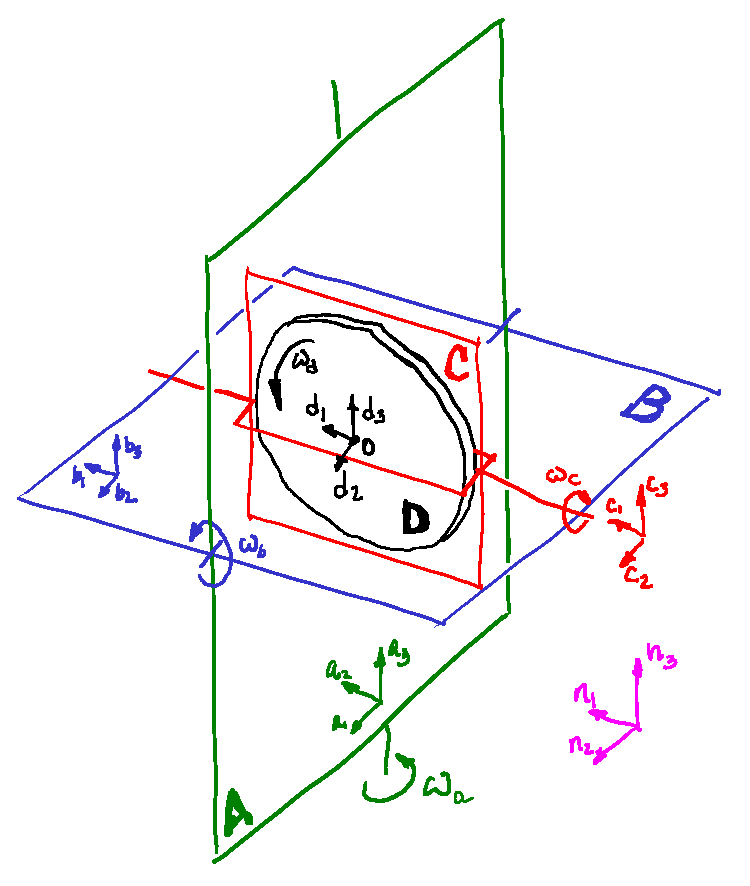
\includegraphics[width=.5\linewidth]{cmg750}
\caption{Control moment gyroscope consists of four rotating bodies: $A, B, C$ and $D$.}
\label{fig:cmg750}
\end{figure}

Пусть у нас есть гиродин, который представляет собой вращающийся диск $D$ внутри трёх рамок $A,B,C$ (рисунок~\ref{fig:cmg750}).
Для начала давайте предположим, что все рамки симметричные, и центры масс всех рамок и диска совпадают в точке $O$.
Таким образом мы можем игнорировать силу тяжести (нет потенциальной энергии) и рассматривать только вращения (в кинетической энергии нет линейных скоростей).

В каждом шарнире у нас есть датчик положения, поэтому мы можем измерять углы $q_d, q_c, q_b, q_a$, которые полностью определяют конфигурацию системы.
Положение при нулевых углах нарисовано на рисунке~\ref{fig:cmg750}.
Заодно введём обозначение угловых скоростей: $\dot{q}_a = \omega_a$,  $\dot{q}_b = \omega_b$,  $\dot{q}_c = \omega_c$,  $\dot{q}_d = \omega_d$.
Зафиксируем неподвижный репер $\{O, \vec{n}_1, \vec{n}_2, \vec{n}_3\}$, и ``вморозим'' в каждое из четырёх тел $A,B,C,D$ реперы
$\{O, \vec{a}_1, \vec{a}_2, \vec{a}_3\}$,
$\{O, \vec{b}_1, \vec{b}_2, \vec{b}_3\}$,
$\{O, \vec{c}_1, \vec{c}_2, \vec{c}_3\}$,
$\{O, \vec{d}_1, \vec{d}_2, \vec{d}_3\}$.
Давайте определим четыре матрицы преобразования реперов между собой:
$$
R_{na} = \begin{bmatrix}
 \cos(q_a) & \sin(q_a) & 0\\
-\sin(q_a) & \cos(q_a) & 0\\
0         & 0        & 1
\end{bmatrix}
\hspace{1cm}
R_{ab} = \begin{bmatrix}
\cos(q_b) & 0 & -\sin(q_b)\\
0         & 1 &  0        \\
\sin(q_b) & 0 &  \cos(q_b)
\end{bmatrix}
$$

$$
R_{bc} = \begin{bmatrix}
1 &  0         & 0        \\
0 &  \cos(q_c) & \sin(q_c)\\
0 & -\sin(q_c) & \cos(q_c)
\end{bmatrix}
\hspace{1cm}
R_{cd} = \begin{bmatrix}
\cos(q_d) & 0 & -\sin(q_d)\\
0         & 1 &  0        \\
\sin(q_d) & 0 &  \cos(q_d)
\end{bmatrix}
$$

Определим скаляры $I_x,J_x,K_x~(x=a,b,c,d)$ как моменты инерции при вращении вокруг оси $k$ каждого тела соответственно.
Из-за симметрии рамок произведение моментов не рассматриваем, поэтому матрицы инерции будут диагональными.
Тогда кинетическая энергия рамки $A$ может быть записана как:
$$
T_a = \frac{1}{2}\vec\omega_{an}^\top \begin{bmatrix}I_a&0&0\\0&J_a&0\\0&0&K_a\end{bmatrix}\vec\omega_{an},\hspace{1cm}
\vec \omega_{an} := R_{na}\begin{bmatrix}0\\0\\\omega_a\end{bmatrix},
$$
где $\omega_a$ - это угловая скорость вращения рамки $A$ относительно неподвижной системы координат.
Аналогично определяются и кинетические энергии оставшихся трёх тел:
\begin{align*}
T_b = \frac{1}{2}\vec\omega_{bn}^\top \begin{bmatrix}I_b&0&0\\0&J_b&0\\0&0&K_b\end{bmatrix}\vec\omega_{bn},\\
T_c = \frac{1}{2}\vec\omega_{cn}^\top \begin{bmatrix}I_c&0&0\\0&J_c&0\\0&0&K_c\end{bmatrix}\vec\omega_{cn},\\
T_d = \frac{1}{2}\vec\omega_{dn}^\top \begin{bmatrix}I_d&0&0\\0&J_d&0\\0&0&K_d\end{bmatrix}\vec\omega_{dn}, 
\end{align*}
где полные (векторные) угловые скорости $\vec\omega_{bn}$, $\vec\omega_{cn}$ и $\vec\omega_{dn}$ определяются как (векторные) суммы частичных угловых скоростей следующим образом:
$$
\begin{array}{rrrrl}
\vec \omega_{bn}  := &             R_{ab}R_{na}\begin{bmatrix}0\\0\\\omega_a\end{bmatrix} &+             \begin{bmatrix}0\\\omega_b\\0\end{bmatrix} & &\\
\vec \omega_{cn}  := &       R_{bc}R_{ab}R_{na}\begin{bmatrix}0\\0\\\omega_a\end{bmatrix} &+       R_{bc}\begin{bmatrix}0\\\omega_b\\0\end{bmatrix} &+ \begin{bmatrix}\omega_c\\0\\0\end{bmatrix}&\\
\vec \omega_{dn}  := & R_{cd}R_{bc}R_{ab}R_{na}\begin{bmatrix}0\\0\\\omega_a\end{bmatrix} &+ R_{cd}R_{bc}\begin{bmatrix}0\\\omega_b\\0\end{bmatrix} &+ R_{cd}\begin{bmatrix}\omega_c\\0\\0\end{bmatrix} &+ \begin{bmatrix}\omega_d\\0\\0\end{bmatrix}\\
\end{array}
$$

Таким образом, в отсутствие силы тяжести, Лагранжиан будет равен просто кинетической энергии:

$$
L = T_a + T_b + T_c + T_b.
$$

\subsection{Зафиксируем один шарнир}

Например, выпишем его явно при зафиксированном угле $q_b=\omega_b=0$ (я ещё использовал симметрию диска $K_d=I_d$):
$$
L=\frac{1}{2}J_d \omega_d^2 + \frac{1}{2}(I_c+I_d) \omega_c^2 + \frac{1}{2}\left(K_a+J_c+J_d+K_b - (J_c+J_d-K_c-I_d) \cos^2(q_c)\right) \omega_a^2 + J_d \sin(q_c) \omega_d \omega_a
$$

Обозначим для удобства $J_1:=J_c+J_d-K_c-I_d$ и $J_2:=K_a+J_c+J_d+K_b$, тогда лагранжиан будет выглядеть так:
$$
L=\frac{1}{2}J_d \omega_d^2 + \frac{1}{2}(I_c+I_d) \omega_c^2 + \frac{1}{2}\left(J_2 - J_1 \cos^2(q_c)\right) \omega_a^2 + J_d \sin(q_c) \omega_d \omega_a
$$


Что не может не радовать, это уравнение совпадает с уравнением (3.1) из ``\href{http://www.mate.tue.nl/mate/pdfs/9731.pdf}{Explicit solution of the ODEs describing the 3 DOF Control Moment Gyroscope}''.

Напоминалка про уравнения Лагранжа:
$$
\frac{d}{dt}\left(\frac{\partial\mathcal L}{\partial\dot q_i}\right) - \frac{\partial\mathcal L}{\partial q_i} = \tau_i
$$

Для удобства выпишем все частные производные:
\begin{align*}
\frac{\partial\mathcal L}{\partial\omega_d} &=  J_d \omega_d + J_d \sin(q_c) \omega_a & \frac{\partial\mathcal L}{\partial q_d} & =  0\\
\frac{\partial\mathcal L}{\partial\omega_c} &= (I_d+I_c)\omega_c                      & \frac{\partial\mathcal L}{\partial q_c} &= J_d \cos(q_c) \omega_a \omega_d + \frac{1}{2}J_1  \sin(2 q_c) \omega_a^2  \\
\frac{\partial\mathcal L}{\partial\omega_a} &= \left(J_2 - J_1 \cos^2(q_c)\right) \omega_a  + J_d \sin(q_c) \omega_d  & \frac{\partial\mathcal L}{\partial q_a}   &= 0\\
\end{align*}

Если приложить моменты $\tau_d$ и $\tau_c$ в соответствующих шарнирах, тогда уравнения движения примут следующий вид:
\begin{align*}
 J_d \dot\omega_d + J_d \sin(q_c)\dot \omega_a + J_d \cos(q_c)\omega_c\omega_a &=\tau_d\\
(I_d+I_c)\dot\omega_c - J_d \cos(q_c) \omega_a \omega_d - \frac{1}{2}J_1  \sin(2 q_c) \omega_a^2  &= \tau_c \\
\left(J_2 - J_1 \cos^2(q_c)\right)\dot \omega_a + J_1 \sin(2 q_c)\omega_c\omega_a +  J_d \sin(q_c) \dot\omega_d + J_d \cos(q_c) \omega_c\omega_d &= 0\\
\end{align*}

Эти уравнения опять-таки совпадают с процитированной ранее статьёй (ну, за исключением трения в шарнире рамки $A$).
Положим скорость вращения диска $D$ постоянной ($\dot\omega_d=0$), таким образом, у нас остаётся две степени свободы: $q_c$ и $q_a$.
Приведём уравнения к каноническому виду:

$$
\left\{\begin{array}{rl}
\dot q_a &= \omega_a \\
\dot q_c &= \omega_c \\
\dot\omega_c &= \frac{\tau_c + J_d \cos(q_c) \omega_a \omega_d + \frac{1}{2}J_1  \sin(2 q_c) \omega_a^2}{I_d+I_c} \\
\dot\omega_a &= \frac{- J_1 \sin(2 q_c)\omega_c\omega_a - J_d \cos(q_c) \omega_c\omega_d}{J_2 - J_1 \cos^2(q_c)} \\
\end{array}\right.
$$

Глядя на уравнения, я предчувствую, что стартуя из состояния $q_a(0)=\omega_a(0)=\omega_c(0)=0$, $q_c(0)=\pi/2$, то какой бы ни был знак прикладываемого момента $\tau_c$,
рамка $A$ будет ускоряться в одну и ту же сторону.


\end{document}
